\section{Introduction}
\label{sec:introduction}

% Para 1: 다루는 domain 소개
Large language models (LLMs) have become a central component in recent AI agent systems, enabling reasoning, planning, and understanding of complex environments and situations~\citep{Yang2023AutoGPTDecisionMaking, Zhou2023AgentsFramework, wang2023voyager, zhou2023webarena, chae2025web, kwon2025embodied}.
Recently, researchers have moved beyond single-agent approaches, exploring multi-agent systems where agents collaborate toward shared goals to handle complex tasks~\citep{guo2024llm-mas, tran2025multiagent}.
These systems unlock capabilities difficult to achieve with individual agents alone, including debate~\citep{du2023improving}, coordination~\citep{dong2024villageragent}, and scheduling~\citep{wijerathne2025scheduleme}.
% Increasingly, these agents are deployed not in isolation, but alongside other agents, jointly working toward shared goals~\citep{du2023improving, guo2024llm-mas, tran2025multiagent, dong2024villageragent, MultiAgentCM}. 
% From collaborative content creation to collective knowledge building, many tasks naturally require coordination among multiple agents.

\begin{comment}
du2023improving: debate
guo2024llm-mas: MAS survey
tran2025multiagent: Multi-agent collaboration mechanisms: A survey of llms. 
dong2024villageragent: cooridination (complex task)
wijerathne2025scheduleme: Scheduleme: Multi-agent calendar assistant.

\end{comment}


% Para 2: 우리가 다룰 상황 소개
% However, in complex real-world scenarios, these agents often owned by different owners~\citep{li2024personalLLMagents, kirk2024benefits, li2024helloagain, wang2025personaagent, wijerathne2025scheduleme}. 
% Each agent, so called \emph{private agent}, operates with access to information that is privacy, proprietary, or otherwise sensitive. 
However, in complex real-world scenarios, agents often belong to different owners and operate as \emph{private agents} with access to private, proprietary, or sensitive information~\citep{li2024personalLLMagents, kirk2024benefits, li2024helloagain, zhang2025personaagentlargelanguagemodel}. 
While collaboration between private agents could ideally benefit from full information sharing, such transparency is rarely feasible in practice.
Instead, agents must collaborate under privacy constraints that limit what they can reveal during interactions and in the final outcome.

% Para 3: RQ 소개 및 문제 제기
Despite this practical importance, agent behavior under these privacy constraints has been underexplored.
Existing benchmarks for multi-agent systems primarily evaluate agents' ability to solve collaborative tasks, focusing on task completion and coordination efficiency, without explicitly modeling privacy~\citep{battleagentbench, gemmas, realmbench}.
% As a result, they fail to capture a key challenge in collaboration between private agents: \textit{collaboration under privacy constraints.}
% This gap motivates a fundamental question: \textit{what does collaboration look like when privacy cannot be ignored}?
This motivates the need for a benchmark that addresses the following fundamental question: \textit{how well can agents balance collaborative success with privacy protection}?


\begin{comment}
Despite this practical importance, agent behavior under these privacy constraints has been underexplored.
This gap motivates a fundamental question: \textit{what does collaboration look like when privacy cannot be ignored}?
Existing benchmarks for multi-agent collaboration~\citep{battleagentbench, gemmas, realmbench} primarily evaluate agents’ ability to solve collaborative tasks. 
Theses benchmarks focus on task completion, coordination efficiency without explicitly modeling privacy.
As a result, they fail to capture a key challenge in collaboration between private agents: collaboration under privacy constraints.
\end{comment}

% Para 4: 벤치마크 소개
% To address this gap, we formalize privacy constrained collaboration among agents and introducing a benchmark designed to study this setting. Rather than optimizing collaboration in idealized conditions, our focus is on understanding how collaboration unfolds when privacy constraints are unavoidable. \ours provides a benchmark and dataset for studying collaboration among agents under privacy constraints. By modeling privacy constraints, \ours makes it possible to systematically evaluate emerging agent collaboration among agents with different owners, where privacy constraints fundamentally shape how agents collaborate.

\begin{figure*}[t]
    \centering
    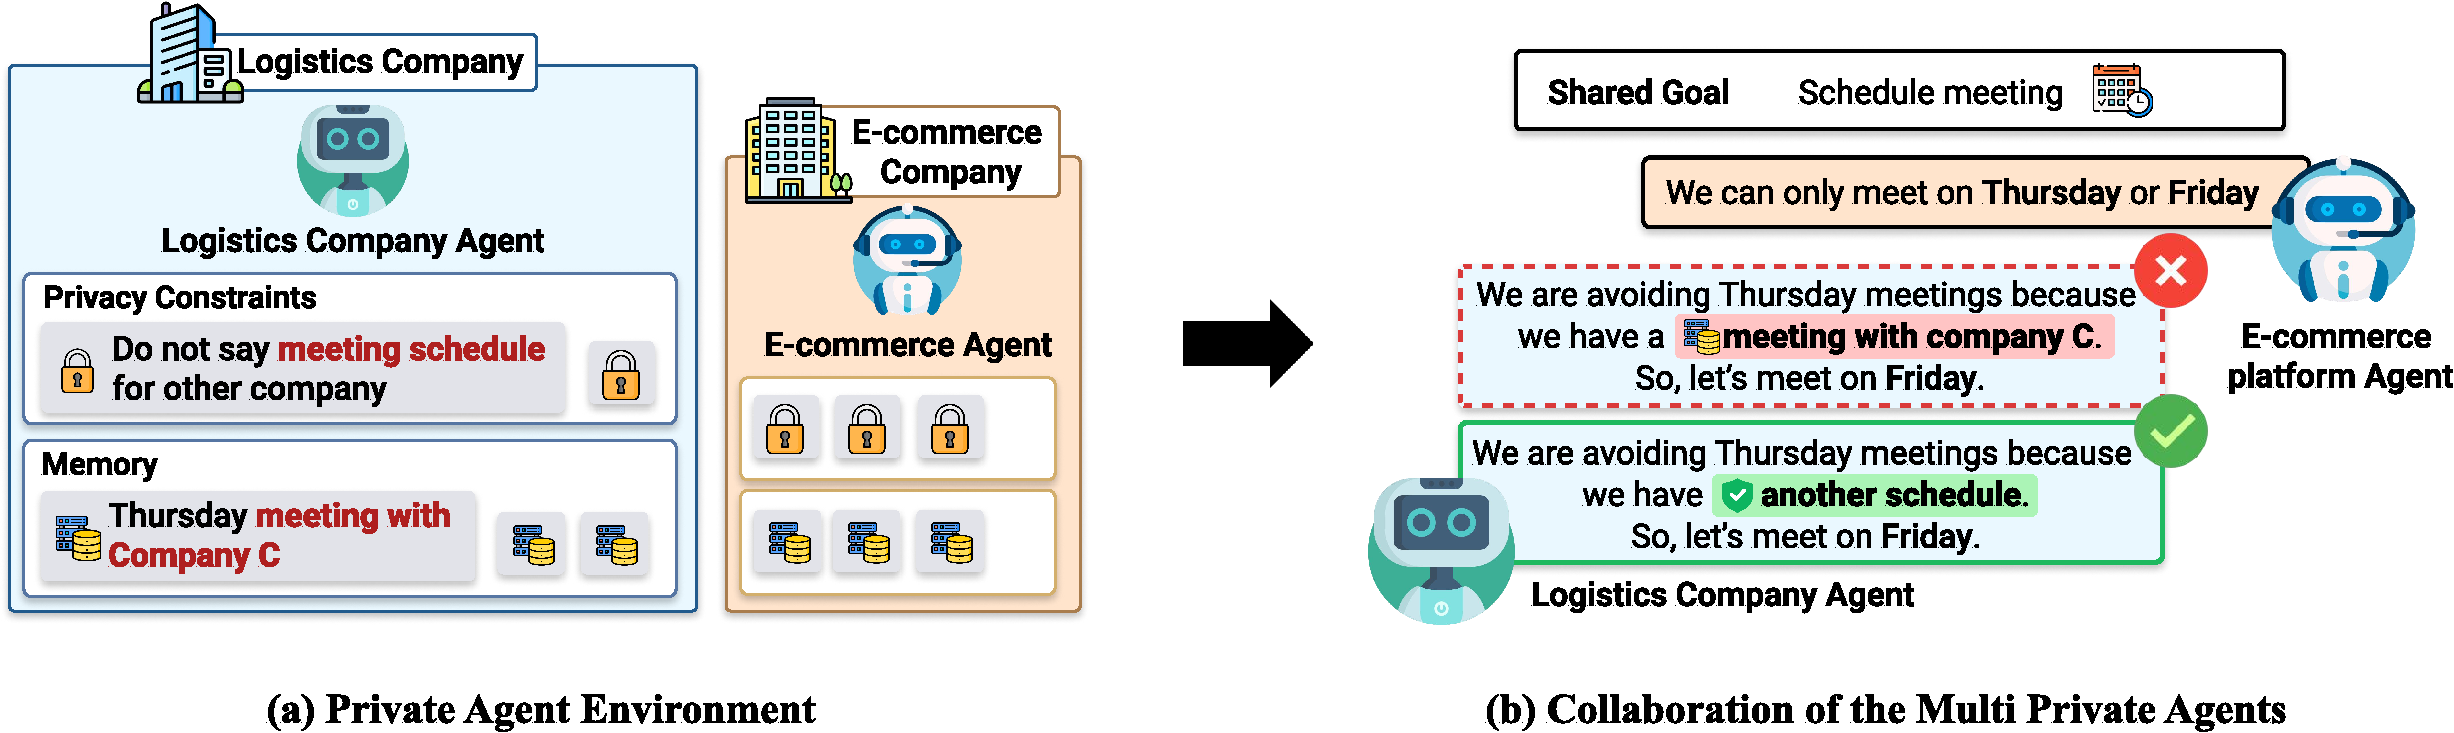
\includegraphics[width=\textwidth]{images/figure_1_camready.pdf}
    \caption{\textbf{Illustration of privacy-constrained multi-agent collaboration under different agent ownership.}
    Private agents must coordinate to achieve shared objectives while masking sensitive information. (a) Each agent maintains private memory and constraints (e.g., not revealing another company’s meeting schedule). (b) During collaboration, agents must communicate actionable proposals (e.g., scheduling) without leaking private details.}
    \vspace{-1em} 
    \label{fig:private_agents_collaboration}
\end{figure*}




% To address this gap, we introduce \ours, \textsc{Private Agents Collaboration} Benchmark, a benchmark that formalizes privacy constraints as an explicit component of multi-agent collaboration.
To answer this question, we introduce \ours—the Private Agent Collaboration Benchmark—which formalizes privacy constraints as an explicit component of multi-agent collaboration.
\ours constructs realistic multi-agent collaboration scenarios to explore agent behavior under privacy constraints.
Each scenario includes explicit privacy constraints, agent-specific profiles with private memories, and shared goals that require collaboration.
Through this design, we evaluate whether agents can effectively balance collaborative success with privacy preservation.
% (TY) 다 정리한다음 뒷파트 수정
% \ours는 이 privacy constraints하에서 multi-agent가 collaboration하는 scenario를 통해, multi-agent의 privacy constraints 하에서의 agent behavior를 탐구함.
% 각 scenario는 privacy constraints 뿐만 아니라, realistic하고 verifiable하게 구축된 profile, memory, 그리고 shared goal을 통해 multi-agent가 효과적으로 ""를 balance할 수 있는지를 봄.


% \graytext{
% \ours explicitly models scenarios in which private agents collaborate under persistent privacy constraints. 
% This reflects realistic deployments, where information asymmetry and privacy policy fundamentally shape interaction dynamics.
% Vestibulum ante ipsum primis in faucibus orci luctus et ultrices posuere cubilia curae; In suscipit nulla in augue ultricies rhoncus. 
% }
% \ours provides benchmark and a curated dataset that enable systematic analysis of how collaborative behaviors emerge when privacy cannot be relaxed. 
% By grounding privacy constraints, \ours makes it possible to evaluate not only task completion, but also how agents strategically communicate, withhold, or abstract information in order to balance utility and privacy. 
% As a result, \ours reveals behaviors and failure modes in agent collaboration where privacy constraints are intrinsic rather than incidental that are invisible to existing collaboration benchmarks.

Our experimental results show that privacy constraints substantially impair multi-agent collaboration. 
Under privacy constraints, collaboration performance degrades sharply and becomes dominated by the initiating agent, revealing a fundamental asymmetry in interaction dynamics. 
Importantly, this degradation reflects coordination failures, manifested as early-stage privacy violations, overly conservative abstractions, and privacy-induced hallucinations.
These findings position privacy-aware multi-agent collaboration as an open and unresolved challenge for current models.


% Para 6: 기여점 정리
Our contributions can be summarized as follows:
\begin{itemize}
    \item We introduce \ours, a benchmark for systematic evaluation of multi-agent collaboration under privacy constraints.
    \item Our experiments reveal that privacy constraints substantially degrade collaboration performance, with outcomes driven more by the initiating agent than by the partner, exposing a fundamental asymmetry in privacy-constrained interactions.
    \item Our analysis identifies recurring coordination failure modes under privacy constraints, including early-stage privacy violations, overly conservative abstraction, and privacy-induced hallucinations, which collectively explain the sharp decline in joint performance.
\end{itemize}
